\subsection{\PovertyMap}\label{sec:app_povertymap}

A different application of satellite imagery is poverty estimation across different spatial regions, which is essential for targeted humanitarian efforts in poor regions \citep{abelson2014poor,epsey2015development}.
However, ground-truth measurements of poverty are lacking for much of the developing world, as field surveys are expensive~\citep{blumenstock2015poverty,xie2016transfer,jean2016combining}.
For example, at least 4 years pass between nationally representative consumption or asset wealth surveys in the majority of African countries, with seven countries that had either never conducted a survey or had gaps of over a decade between surveys~\citep{yeh2020poverty}.
One approach to this problem is to train ML models on countries with ground truth labels and then deploy them to different countries where we have satellite data but no labels.

We study this problem through a variant of the poverty mapping dataset collected by \citet{yeh2020poverty}.

\subsubsection{Setup}

\paragraph{Problem setting.}
We consider a hybrid domain generalization and subpopulation shift problem,
where the input $x$ is a multispectral LandSat satellite image with 8 channels (resized to 224 $\times$ 224 pixels),
the output $y$ is a real-valued asset wealth index computed from Demographic and Health Surveys (DHS) data, and the domain $d$ represents the country the image was taken in and whether the image is of an urban or rural area.
We aim to solve both a domain generalization problem across country borders and improve subpopulation performance across urban and rural areas.

\paragraph{Data.}
\PovertyMap is based on a dataset collected by~\citet{yeh2020poverty}, which assembles satellite imagery and survey data at 19,669 villages from 23 African countries between 2009 and 2016 (Figure~\ref{fig:dataset_poverty}).
Each input image has 8 channels: 7 from the LandSat satellite and an 8th channel for nighttime light intensity from a separate satellite,
as prior work has established that these night lights correlate with poverty measures~\citep{noor2008nighttime,elvidge2009poverty}.

There are $23 \times 2 = 46$ domains corresponding to the 23 countries and whether the location is urban or rural.
Each example comes with metadata on its location coordinates, survey year, and its urban/rural classification.

In contrast to other datasets, which have a single fixed ID/OOD split, the relatively small size of \PovertyMap allows us to use 5 different folds, where each fold defines a different set of OOD countries.
In each fold, we use the following splits of the data (the number of countries and images in each split varies slightly from fold to fold):
\begin{enumerate}
    \item \textbf{Training:} $\sim$10000 images from 13--14 countries.
    \item \textbf{Validation (OOD):} $\sim$4000 images from 4--5 different countries (distinct from training and test (OOD) countries).
    \item \textbf{Test (OOD):} $\sim$4000 images from 4--5 different countries (distinct from training and validation (OOD) countries).
    \item \textbf{Validation (ID):} $\sim$1000 images from the same 13--14 countries in the training set.
    \item \textbf{Test (ID):} $\sim$1000 images from the same 13--14 countries in the training set.
\end{enumerate}
All splits contain images of both urban and rural locations, with the countries assigned randomly to each split in each fold.

The distribution of wealth may shift across countries due to differing levels economic development, agricultural practices, and other factors. For example, \citet{abelson2014poor} use thatched vs. metal roofs to distinguish between poor and wealthy households, respectively in Kenya and Uganda. However, other countries may have a different mapping of roof type to wealth where metal roofs signify more poor households. Similar issues can arise when looking at the health of crops (related to vegetation indices such as NDVI that are simple functions of the multispectral channels in the satellite image) as a sign for wealth in rural areas, since crop health is related to climate and the choice of crops, which vary upon region.

Asset wealth may also shift dramatically between countries. Figure~\ref{fig:poverty-wealth-by-splits} shows the mean asset wealth per country, as well as urban vs. rural asset wealth per country.
Mean asset wealth ranges from -0.4 to +0.8 depending on the country.
There is a stark difference between mean asset wealth in urban and rural areas, with urban asset wealth being positive in all countries while rural mean asset wealth being mostly negative.

\begin{figure*}[tbp]
  \centering
  \begin{subfigure}{0.48\textwidth}
      \centering
      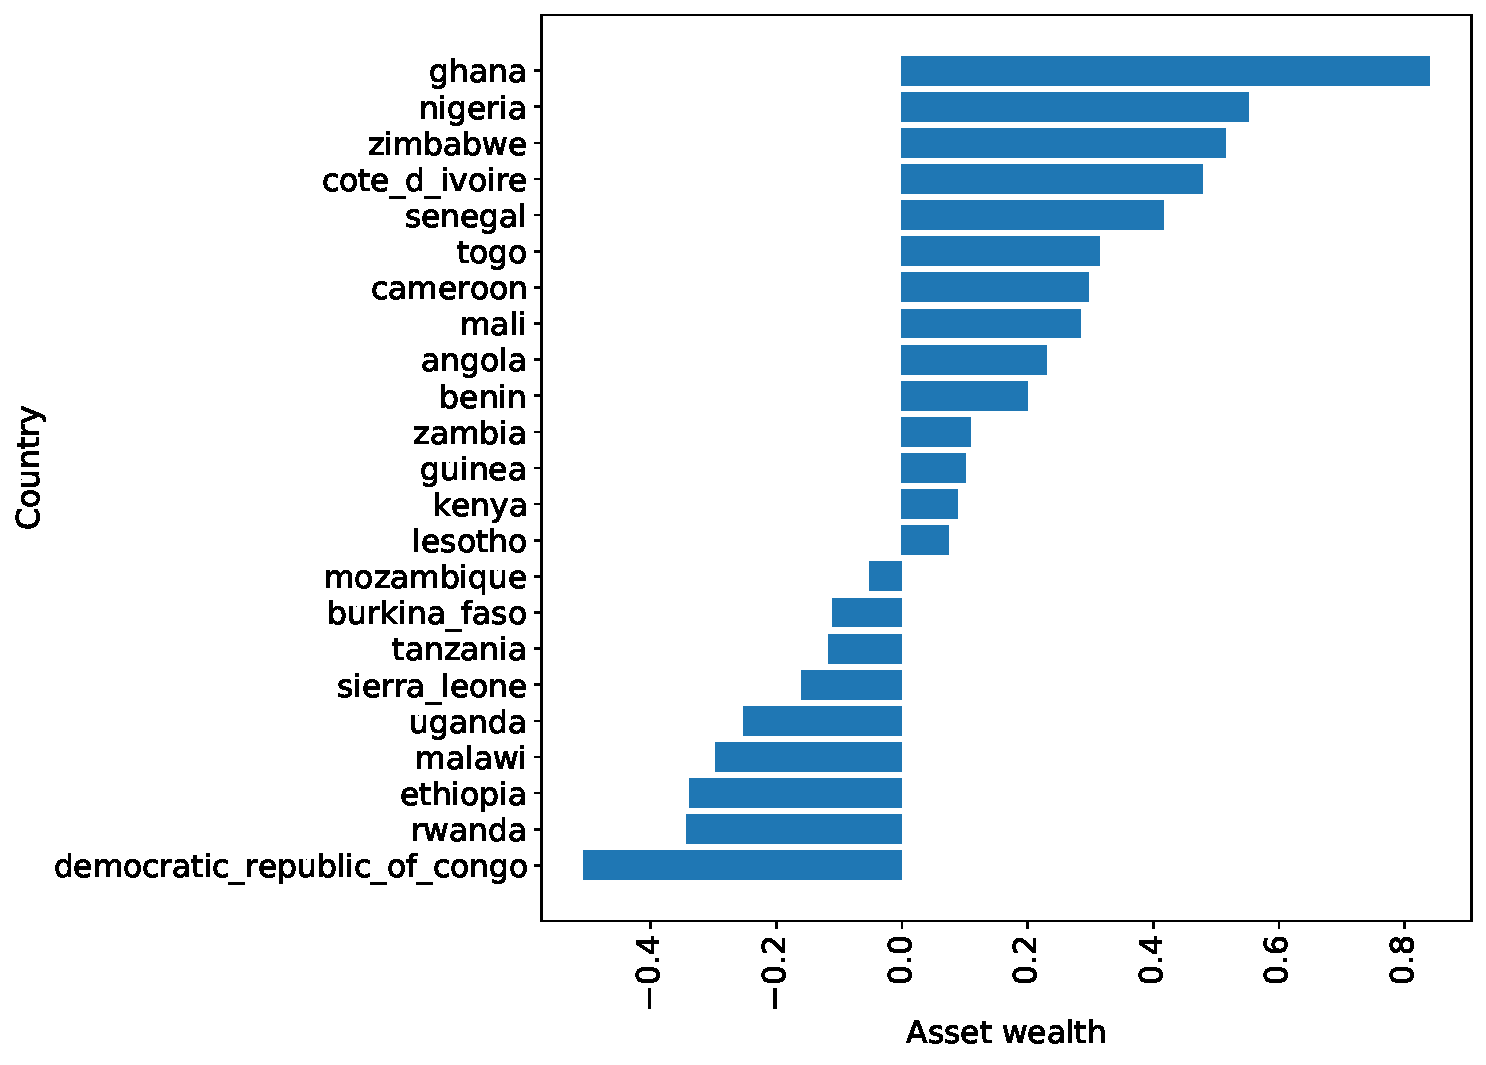
\includegraphics[width=\textwidth]{figures/poverty_wealth_per_country.pdf}
    \end{subfigure}
    \hfill
    \begin{subfigure}{0.48\textwidth}
      \centering
      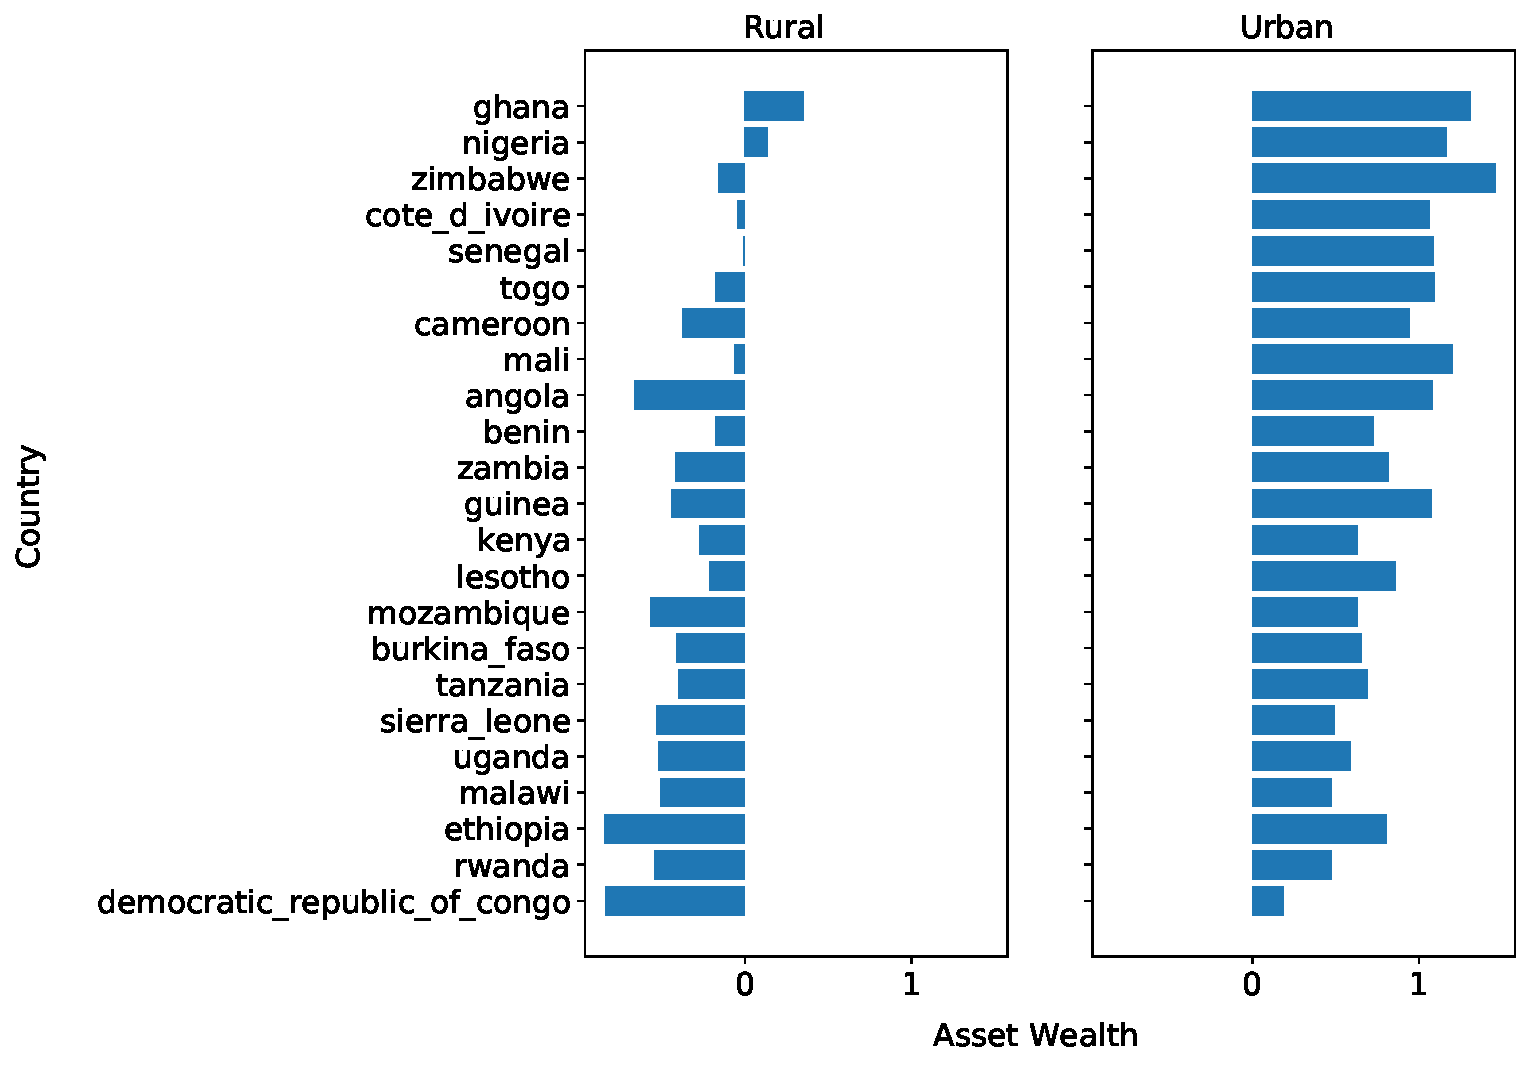
\includegraphics[width=\textwidth]{figures/poverty_wealth_per_country_urbanrural.pdf}
    \end{subfigure}
  \caption{Mean asset wealth by country on aggregate as well as urban and rural splits for each country, computed on the full dataset.}\label{fig:poverty-wealth-by-splits}
\end{figure*}

\paragraph{Evaluation.}
As is standard in the literature~\citep{jean2016combining,yeh2020poverty}, the models are evaluated on the Pearson correlation ($r$) between their predicted and actual asset wealth indices.
We measure the average correlation, to test generalization under country shifts, and also the lower of the correlations on the urban and rural subpopulations, to test generalization between urban and rural subpopulations.
We report the latter as previous works on poverty prediction from satellite imagery have noted that a significant part of model performance relies on distinguishing urban vs. rural areas, and improving performance within these subpopulations is an ongoing challenge, with rural areas generally faring worse under existing models~\citep{jean2016combining,yeh2020poverty}.

We average all correlations across the 5 different folds, using 1 random seed per fold. The resulting standard deviations reflect the fact that different folds have different levels of difficulty (e.g., depending on how similar the ID and OOD countries are).
For the purposes of comparing different algorithms and models, we note that these standard deviations might make the comparisons appear noisier than they are, since a model might perform similarly across random seeds but still have a high standard deviation if it has different performances on different folds on the data.
In contrast, other \Wilds datasets report results on the same data split but averaged across different random seeds.

\paragraph{Potential leverage.}
Large socioeconomic differences between countries makes generalization across borders challenging. However, some indicators of wealth are known to be robust and are able to be seen from space. For example, roof type (e.g. thatched or metal roofing) has been shown to be a reliable proxy for wealth~\citep{abelson2014poor}, and contextual factors such as the health of nearby croplands, the presence of paved roads, and connections to urban areas are plausibly reliable signals for measuring poverty.
Poverty measures are also known to be highly correlated across space, meaning nearby villages will likely have similar poverty measures, and methods can utilize this spatial structure (using the provided location coordinate metadata) to improve predictions~\citep{jean2018ssdkl,rolf2020post}.
We show the correlation with distance in Figure~\ref{fig:poverty-wealth-distance}, which plots the distance between pairs of data points against the absolute differences in asset wealth between pairs.

\begin{figure}[tbp]
  \centering
  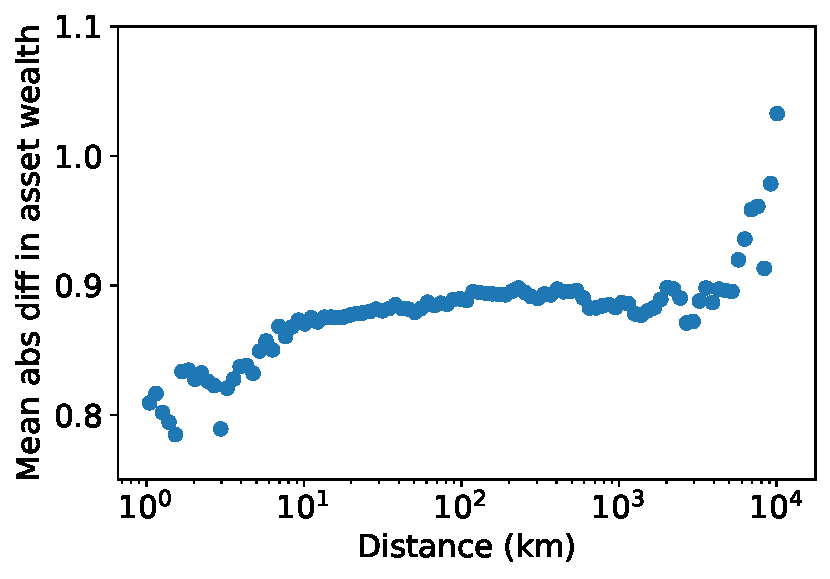
\includegraphics[width=0.5\linewidth]{figures/poverty_wealth_by_distance.pdf}
  \caption{Mean absolute difference in asset wealth between two data points in the full dataset as a function of (great circle) distance between the two points. Smaller distances between data points correlate with more similar asset wealth measures. The pairs are binned by distance on a log (base 10) scale (100 bins), and the mean value of each bin is plotted at the midpoint distance of each bin.}\label{fig:poverty-wealth-distance}
\end{figure}


\subsubsection{Baseline results}
\paragraph{Model.}
For all experiments, we follow \citet{yeh2020poverty} and train a ResNet-18 model \citep{he2016resnet} to minimize squared error.
We use the Adam optimizer \citep{kingma2014adam} with an initial learning rate of $10^{-3}$ that decays by 0.96 per epoch, and train for 200 epochs for with early stopping (on OOD $r$) and with a batch size of 64.


\paragraph{ERM results and performance drops.}
When shifting across country borders, Table~\ref{table:poverty-map} shows that ERM suffers a 0.04 drop in average $r$ in the official OOD setting compared to the train-to-train ID setting.
Moreover, the drop in performance is exacerbated when looking at urban and rural subpopulations, even though all splits contain urban and rural examples;
the difference in worst $r$ over the urban and rural subpopulations triples from 0.04 to 0.12 compared to the difference in average $r$.
Correlation is consistently lower on the rural subpopulation than the urban subpopulation.

We ran an additional mixed-to-test comparison where we considered an alternative training set with data that was uniformly sampled from all countries, while keeping the overall training set size constant (i.e., compared to the standard training set, it has fewer examples from each country, but data from more countries).
A model trained on this mixed split had a much smaller drop in performance between the ID and OOD test sets (Table~\ref{table:poverty-map-compare}), which implies that the performance drop between the ID and OOD test sets is largely due to the distribution shift from seen to unseen countries.

\begin{table*}[tbp]
\caption{Pearson correlation $r$ (higher is better) on in-distribution and out-of-distribution (unseen countries) held-out sets in \PovertyMap, including results on the rural subpopulations.
ID results correspond to the train-to-train setting.
All results are averaged over 5 different OOD country folds taken from~\citet{yeh2020poverty}, with standard deviations across different folds in parentheses.}
  \centering
\begin{tabular} {l r r r r}
\toprule
 & Validation (ID) & Validation (OOD) & Test (ID) & Test (OOD)\\
\midrule
Overall & & & &\\
~~~~ERM & 0.82 (0.02) & 0.80 (0.04) & 0.82 (0.03) & \textbf{0.78} (0.04)\\
~~~~CORAL & 0.82 (0.00) & 0.80 (0.04) & \textbf{0.83} (0.01) & 0.78 (0.05)\\
~~~~IRM & 0.82 (0.02) & 0.81 (0.03) & 0.82 (0.02) & 0.77 (0.05)\\
~~~~Group DRO  & 0.78 (0.03) & 0.78 (0.05) & 0.80 (0.03) & 0.75 (0.07) \\
Worst urban/rural subpop & & & &\\
~~~~ERM & 0.58 (0.07) & 0.51 (0.06) & 0.57 (0.07) & \textbf{0.45} (0.06)\\
~~~~CORAL & 0.59 (0.04) & 0.52 (0.06) & \textbf{0.59} (0.03) & 0.44 (0.06) \\
~~~~IRM & 0.57 (0.06) & 0.53 (0.05) & 0.57 (0.08) & 0.43 (0.07)\\
~~~~Group DRO  & 0.49 (0.08) & 0.46 (0.04) & 0.54 (0.11) & 0.39 (0.06) \\
\bottomrule
\end{tabular}
\label{table:poverty-map}
\end{table*}

\begin{table*}[!h]
  \caption{Mixed-to-test comparison for ERM models on \PovertyMap.
  In the official OOD setting, we train on data from one set of countries, and then test on a different set of countries.
  In the mixed-to-test setting, we train on the same amount of data but sampled uniformly from all countries, and then test on data from the same countries as in the official setting.
  The Test (ID) and Test (OOD) sets used for the mixed-to-test results are smaller (subsampled at random) than those used for the official results, as some test examples were used for the training set in the mixed-to-test setting.
  Models trained on the official split degrade in performance, especially on rural subpopulations,
  while models trained on the mixed-to-test split do not.}
  \centering
\begin{tabular} {l l r r r r r r}
\toprule
& \multicolumn{3}{c}{Test (ID)} & \multicolumn{3}{c}{Test (OOD)} \\
Setting & Overall $r$ & Rural $r$ & Urban $r$ & Overall $r$ & Rural $r$ & Urban $r$\\
\midrule
  Official & 0.82 (0.03) & 0.57 (0.07) & 0.66 (0.04) & 0.78 (0.04) & 0.46 (0.05) & 0.59 (0.11) \\
  Mixed-to-test & 0.83 (0.02) & 0.61 (0.08) & 0.65 (0.06) & 0.83 (0.03) & 0.60 (0.06) & 0.65 (0.06)\\
\bottomrule
\end{tabular}
\label{table:poverty-map-compare}
\end{table*}

\paragraph{Additional baseline methods.}
We trained models with CORAL, IRM, and Group DRO, taking examples from different countries as coming from distinct domains.
Table~\ref{table:poverty-map} shows that these baselines are generally comparable to ERM and that they continue to be susceptible to shifts across countries and urban/rural areas.
As with most other datasets, our grid search selected the lowest values of the penalty weights for CORAL ($\lambda = 0.1$) and IRM ($\lambda = 1$).

\paragraph{Discussion.}
These results corroborate performance drops seen in previous out-of-country generalization tests for poverty prediction from satellite imagery~\citep{jean2016combining}.
In general, differences in infrastructure, economic development, agricultural practices, and even cultural differences can cause large shifts across country borders.
Differences between urban and rural subpopulations have also been well-documented~\citep{jean2016combining,yeh2020poverty}. Models based on nighttime light information could suffer more in rural areas where nighttime light intensity is uniformly low or even zero.

Since survey years are also available, we could also investigate the robustness of the model over time. This would enable the models to be used for a longer time before needing more updated survey data, and we leave this to future work. \citet{yeh2020poverty} investigated predicting the change in asset wealth for individual villages in the World Bank Living Standards Measurement Surveys (LSMS), which is a longitudinal study containing multiple samples from the same village.
\PovertyMap only contains cross-sectional samples which do not provide direct supervision for changes over time at any one location, but it is still possible to consider aggregate shifts across years.

As with \FMoW, there are important ethical considerations associated with remote sensing applications,
e.g., around surveillance and privacy issues, as well as the potential for systematic biases that negatively affect particular populations.
As we describe in \refsec{app_povertymap_details}, noise has been added to the location metadata in \PovertyMap to protect privacy.
The distribution shifts across country and urban/rural boundaries that we study in \PovertyMap are an example of a bias that affects model performance and therefore could have adverse policy consequences.
We refer interested readers to the UNICEF discussion paper by \citet{berman2018ethical} for a more in-depth discussion of the ethics of remote sensing especially as it pertains to development and humanitarian endeavors.

\subsubsection{Broader context}
Computational sustainability applications in the developing world also include tracking child mortality~\citep{burke2016mortality,osgood2018mapping,reiner2018mortality}, educational attainment~\citep{graetz2018education}, and
food security and crop yield prediction~\citep{you2017crop,wang2020weakly,xie2020innout}.
Remote sensing data and satellite imagery has the potential to enable high-resolution maps of many of these sustainability challenges, but as with poverty measures, ground truth labels in these applications come from expensive surveys or observations from human workers in the field.
Some prior works consider using spatial structure~\citep{jean2018ssdkl,rolf2020post}, unlabeled data~\citep{xie2016transfer,jean2018ssdkl,xie2020innout}, or weak sources of supervision~\citep{wang2020weakly} to improve global models despite the lack of ground-truth data.
We hope that \PovertyMap can be used to improve the robustness of machine learning techniques on satellite data, providing an avenue for cheaper and faster measurements that can be used to make progress on a general set of computational sustainability challenges.

\subsubsection{Additional details}\label{sec:app_povertymap_details}

\paragraph{Data processing.}
The \PovertyMap dataset is derived from~\citet{yeh2020poverty}, which gathers LandSat imagery and Demographic and Health Surveys (DHS) data from 19669 villages across 23 countries in Africa .
The images are $224 \times 224$ pixels large over 7 multispectral channels and an eighth nighttime light intensity channel. The LandSat satellite has a 30m resolution, meaning that each pixel of the image covers a $30m^2$ spatial area.
The location metadata is perturbed by the DHS as a privacy protection scheme; urban locations are randomly displaced by up to 2km and rural locations are perturbed by up to 10km. While this adds noise to the data, having a large enough image can guarantee that the location is in the image most of the time.
The target is a real-valued composite asset wealth index computed as the first principal component of survey responses about household assets, which is thought to be a less noisy measure of households' longer-run economic well-being than other welfare measurements like consumption expenditure~\citep{sahn2003asset,filmer2011asset}.
Asset wealth also has the advantage of not requiring adjustments for inflation or for purchasing power parity (PPP), as it is not based on a currency.

We normalize each channel by the pixel-wise mean and standard deviation for each channel, following~\citep{yeh2020poverty}. We also do a similar data augmentation scheme, adding random horizontal and vertical flips as well as color jitter (brightness factor 0.8, contrast factor 0.8, saturation factor 0.8, hue factor 0.1).

The data download process provided by~\citet{yeh2020poverty} involves downloading and processing imagery from Google Earth Engine. We process each image into a compressed NumPy array with 8 channels. We also provide all the metadata in a CSV format.

\paragraph{Additional results.}
We also ran an ablation where we removed the nighttime light intensity channel.
This resulted in a drop in OOD $r$ of 0.04 on average and 0.06 on the rural subpopulation, demonstrating the usefulness of the nightlight data in asset wealth estimation.

\paragraph{Modifications to the original dataset.}
We report a much larger drop in correlation due to spatial shift than in~\citet{yeh2020poverty}.
To explain this, we note that our data splitting method is slightly different from theirs.
They have two separate experiments (with different data splits) to test in-distribution vs. out-of-distribution generalization.
In contrast, our data splits on both held-out in-distribution and out-of-distribution points at the same time with respect to the same training set, thus allowing us to compare both metrics simultaneously on one model as a more direct comparison.
We use the same OOD country folds as the original dataset.
However,~\citet{yeh2020poverty} split the ID train/val/test while making sure that the spatial extent of the images between each split never overlap,
while we simply take uniformly random splits of the ID data.
This means that between our ID train/val/test splits, we may have images that have share some overlapping spatial extent, for example for two very nearby locations.
Thus, a model can utilize some memorization here to improve ID performance.
We believe this is reasonable since, with more ID data, more of the spatial area will be labeled and memorization should become an increasingly viable strategy for generalization in-domain.
